\documentclass{article}
\usepackage[utf8]{inputenc}
\usepackage[english, polish]{babel}
\usepackage{forloop}
\usepackage[T1]{fontenc}
\usepackage{amsfonts}
\usepackage{tikz}
\usepackage{graphicx}
\usepackage{amsmath}
\usepackage{graphicx}
\title{Lista 9}
\author{Łukasz Magnuszewski}
\date{\vspace{-5ex}}
%\date{} 
\begin{document}

\maketitle

\section*{Zadanie 1}
Przyjmijmy następujące oznacznie
K: koza,
W: Wilk,
S: Sałata,
P: Przewoźnik
Oraz niech | rozdziela to co jest po lewej oraz prawej stronie rzeki.

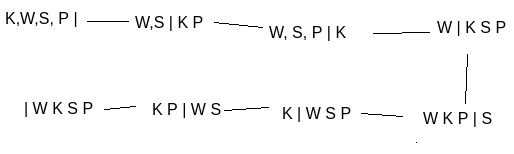
\includegraphics{koza}S
\section*{Zadanie 2}
Będę korzystał ze wzoru
\[
  |G| = |G_x| | O_x|
\]
W Rysunku pierwszym, przyjmijmy następująca numeracje wierzchołków, leksykograficznie według współrzędnych, przy czym nie nadajemy numeru dla x.
\[
  |O_x| = |\{1, 2, x, 6\}| = 4
\]
Bo x może przejść na wszystkie wierzchołki po prawej i lewej stronie.
Zaś 
\[
  |G_x| = |\{id, (1,2), (3,5), (1,2)(3,5)\}| = 4
\]
Więc $|G| = 4 * 4 = 16$


W rysunku drugim przyjmijmy analogiczne oznaczenia. Wtedy
\[
  |O_x| = |\{1, 2, 3, 4, 5, 6, x, 7\}| = 8
\]
Z tego jak spermutujemy sąsiadów x czyli 1, 5, 7 wynikają jednoznacznie rozstawienie pozostałych wierzchołków.
\[
  |G_x| = 3!
\]
Więc $|G| = 8 * 3! = 48$
\section*{Zadanie 3}
Jest to graf 3 regularny więcx może przejśc na każdy wierzchołek
\[
  |O_x| = 10
\]
Zaś 
\[
  |G_x| = 3! 2!
\]
Bo najpierw permutujemy sąsiadów x a potem sąsiadów jednego z sąsiadów x, a reszta jest już wyznaczona jednoznacznie.

\section*{Zadanie 8}
\subsection*{Zależności}
\[
n(Q_k) = 2^k  
\]
Oczywiste, liczba ciągów binarnych długości k.
\[
m(Q_k) = k 2^{k-1}  = k \frac{2^k}{2}
\]
Rozpatrujemy wszystkie możliwe ciągi stąd $2^k$ potem rozpatrujemy wszystkie pozycje na których moze być ta jedyna różnica stąd $k$. A potem dzielimy przez 2 bo to graf nieskierowany.

\subsection*{Dwudzielność}
Niech A będzie takim zbiorem że $\forall a,b \in A$ a oraz b różnią się na parzystej liczbie pozycji. Zaś B niech będzie równe $Q_k \setminus A$. W oczywiste sposób $A \bigcup B = Q_k$.
\subsection*{A}
Oraz to że między dowlnymi wierzchołkami z A nie ma krawędzi. Bo wierzchołki między którymi jest krawędź różnią się na 1 pozycji, czyli jest to nieparzysta liczba różnić.
\subsubsection*{B}
Załóżmy niewprost $\exists x,y \in B$ takie że różnią się na dokładnie jednej pozycji. Ale weźmy wtedy $a \in A$ takie że a różni się z x na tej pozycji, na której x różni się z y. Ale wtedy a z y różnią się na parzystej liczbie pozycji, czyli y należy do A sprzeczność.

\section*{Zadanie 8}
Graf dwudzielny można podzielić na dwa podzbiory wierzchołków A, B takie że $A \bigcup B = V, A \bigcap B = \emptyset$. Czyli $|A| + |B| = |V|$. Wtedy by zmaksymalizować liczbę krawędzi należy z każdego wierzchołka z A poprowadzić krawędź do każdego wierzchołka z B. Czyli maksymlna liczba krawędzi dla danych A i B wynosi $|A| * |B|$. Z prostej optymalizacji wynika że maksymalny wynik jest osiągany dla $|A| = |B|$ dla parzystych oraz $|A| = |B| + 1$ dla nieparzystych. co daje oszacowanie $\lfloor \frac{n^2}{4} \rfloor$


\section*{Zadanie 9}
Załóżmy niewprost że G oraz jego dopełnienie są niespójne.
Wtedy graf G ma przynajmniej 2 spójne. nazwjimy je A, B. Oraz w każdej z tych spójnych jest przynajmniej jeden wierzchołek, nazwijmy je a,b. W dopełnieniu a oraz b są połączone bo w G są w różnych spójnych. Rozważmy teraz wszystkie pozostałe wierzchołki. Może zachodzić jeden z 2 przypadków $x \in A$, wtedy x jest połączony z b w dopełenieniu. W przeciwnym wypadku x jest połączone z a. Czyli pokazaliśmy że dopełnienie grafu jest spójne. Sprzeczność!

\section*{Zadanie 9}
Załóżmy niewprost że istnieją dwie rozłączne najdłuższe ścieżki proste $A, B$. Niech ich długość wynosi n. Ale jako że jest to graf spójny, to między pierwszym wierzchołkiem ścieżki A i pierwszym wierzchołkiem ścieżki B istnieje ścieżka C. Możemy teraz obciąć C tak by pozostał w niej tylko jeden wierzchołek z A oraz B. nazwijmy te wierzchołki a,b. Obcięte c zawiera przynajmniej jedną krawędź. Wierzchołki a,b dzielą ścieżki A, B na dwie części (w szczególności mogą być puste). Przynajmniej jedna z tych części ma długość większą równą od połowy długości orginalnej ścieżki. To jak weźmiemy te większe połówki z A,B i połączymy je obciętym C to wyjdzie nam prosta ścieżka o długości $z \geq \frac{n}{2} * 2 + 1 > n$. Sprzeczność.

\section*{Zadanie 7}
\subsection*{podpunkt a}
\[
  2^{\frac{n(n-1)}{2}}
\]
Najpierw należy policzyć maksymalną liczbę krawędzi nieskierowanych między różnymi wierzchołkami czyli $\frac{n(n-1)}{2}$. I potem każda krawędź albo należy do grafu, albo nie. Czyli podnosimy 2 do potęgi $\frac{n(n-1)}{2}$.
\subsection*{podpunkt b}
Z poprzedniego punktu wiemy że liczba możliwych różnych krawędzi między różnymi wierzchołkami to $\frac{n(n-1)}{2}$. Zaś liczba różnych pętli to n. 


\end{document}



